\secnumbersection{PROPUESTA DE SOLUCIÓN}

\subsection{Identificación de datos deseados}

Los registros de log proporcionan una gran cantidad de información sobre las operaciones del VLT en una noche. Sin embargo, para efectos prácticos no es necesario ingerir toda esta información; acorde al objetivo general, solo se buscan datos relevantes para el sistema de Óptica Activa.

Debido a esto, antes del diseño del procedimiento ETL, es necesario hacer un estudio de los registros de log y determinar aquellos que se tengan importancia dentro del contexto de la Óptica Activa.

Cada telescopio durante su operación nocturna, genera un log sobre su comportamiento. De esta información se deben extraer dos caracteristicas centrales: datos sobre la Óptica Activa y datos sobre las características ambientales.

Los datos principales serán aquellos relacionados con el sistema de Óptica Activa: las distribuciones de fuerzas de los 150 actuadores, las imágenes tomadas durante la operación y las instancias de corrección; todas dentro del rango de una observación.

\subsubsection{Instancia de corrección}

Se realizan varias correcciones de las distribuciones de fuerza en un ciclo de Óptica Activa, cada una de las cuáles se realiza en base a una imágen tomada anteriormente.

Si se toma en consideración que estas correcciones van en serie, entonces cada una de estas es precedida por la distribución de fuerza que corrigieron, y seguida por la nueva imágen capturada por el telescopio.

Con esto en consideración, se puede separar la instancia de la corrección de las distribuciones de fuerza, y de esta forma tener un dato con el cuál poder relacionar las imágenes y las distribuciones de fuerza.

\subsubsection{Distribución de fuerzas}

Para el contexto del sistema de Óptica Activa, se hace necesario conocer los valores de las distribuciones de fuerza de los 150 actuadores, ya que esta es la cantidad que se busca optimizar durante la Óptica Activa \cite{eso1998vlt}. 

Durante cada iteración de la Óptica Activa, se analizan las aberraciones de la imágen tomada previamente y luego se calculan los cambios en los valores de la distribución de fuerza en los actuadores del espejo M1. Finalmente, se suman estas diferencias a la distribución de fuerza en vigencia, terminando en una distribución de fuerza final \cite{wilson1987active}.

Tanto los cambios en la distribución de fuerzas como la distribución final son escritas en los registros de log. Como se busca extraer un conjunto de distribuciones de fuerzas, presentes en el registro de log, se decide extraer la distribución final y descartar los cambios en la distribución de fuerzas.

\subsubsection{Imágenes tomadas}

Durante el proceso de Óptica Activa, las correcciones de las distribuciones de fuerza en los actuadores son realizadas en base a imágenes tomadas previamente por los sensores. Se debe considerar, además, que el proceso es iterativo, por lo que después de una corrección, se toma una nueva imágen con la nueva distribución de fuerzas para una nueva corrección, continuando el ciclo \cite{eso1998vlt}.

Con estas consideraciones en mente, se puede inferir para una instancia de corrección, debe existir una imágen tomada antes y una imágen tomada después, donde esta última correspondería a la imágen previa de la siguiente instancia de corrección.

\subsubsection{Datos adicionales}

Existen otras características ambientales que son de interés, debido a que  podrían estar relacionados con la modificación de la toma de datos desde el espejo.

Debido a esto, se ha generado la siguiente lista de características ambientales que también se deben extraer:

\begin{itemize}
    \item Torque aplicado al motor, tanto en altitud como en acimut, durante el tracking del telescopio \cite{eso1998vlt}.

    \item Posición y ángulo del UT en el momento de la observación, representados ambos con altitud y acimut \cite{eso1998vlt}.

    \item Velocidad y dirección del viento detectado dentro de la estructura del telescopio, medidos en metros por segundo y grados, respectivamente \cite{eso1998vlt}.

    \item Temperatura ambiental detectada dentro de la estructura del telescopio, medida en grados Celsius \cite{eso1998vlt}.

    \item Porcentaje de humedad ambiental relativa detectada dentro de la estructura del telescopio \cite{eso1998vlt}.

    \item Presión del aire detectada dentro de la estructura del telescopio \cite{eso1998vlt}.    
\end{itemize}

\subsection{Almacenamiento de datos}

Una vez identificados los datos a extraer desde las líneas de log, se hace necesario plantear como se almacenaran los mismos despues de obtenerlos. 

Tener esta claridad previo al desarrollo del procedimiento ETL permite tener la claridad de que transformaciones realizar a los datos extraídos.

Para la solución a desarrollar, es presenta una estructura de almacenamiento de datos en la Imágen \ref{fig:db_general}.

\begin{figure}[h]
\centering
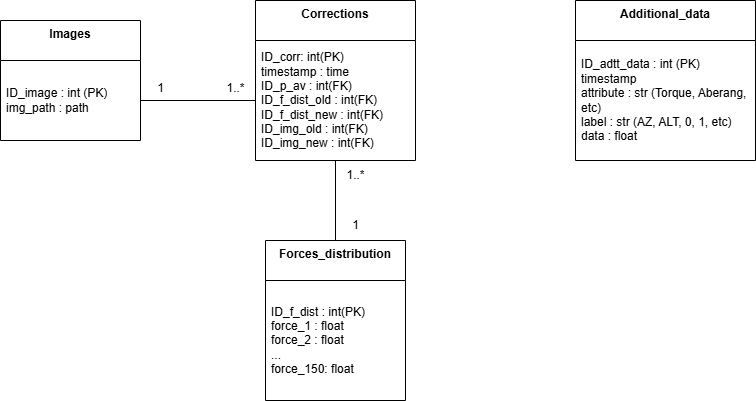
\includegraphics[width=10cm,height=6cm]{figures/db_diagram.png}
\caption{\label{fig:db_general} Malla Curricular Ingeniería Civil Informática.} Fuente: Elaboración propia.
\end{figure}

\subsubsection{Estructura de los datos}

Según lo visto anteriormente, los datos principales consisten en imágenes, distribuciones de fuerzas, etc. asociados a instancias de corrección de la forma del espejo M1. Más específicamente, se tiene que cada instancia de corrección cambia, generalmente, los valores de estos datos. 

Se puede considerar entonces agrupar los datos deseados según la instancia de corrección asociada. Por lo señalado anteriormente, cada instancia de corrección tendría asociado un set de datos previos a la corrección y otro set de datos similar luego de la misma. Entonces, cada corrección correspondería a una tabla con ambos sets de datos como atributos de la misma.

Esto puede llevar a un problema, ya que en el escenario de dos correcciones consecutivas, el set de datos post-corrección de la primera instancia y el set de datos pre-corrección de la segunda instancia serían los mismos, por lo que estos datos aparecen repetidos en ambas tablas.

Para solucionar este problema, una vez agrupados los datos, se opta por separar las correcciones y los sets de datos asociados en tablas distintas pero relacionadas entre sí con llaves foráneas. Al mantener entidades distintas con múltiples relaciones por tabla, se logra normalizar la información.

Siguiendo con el caso anterior, se tendrían dos tablas para las correcciones más tres tablas para los sets de datos: una tabla para el set de datos pre-corrección asociada a la primera corrección, una tabla para el set de datos post-corrección asociada a la segunda corrección y una tercera tabla para el set de datos entre ambas correcciones, a las cuales se relaciona usando llaves foráneas desde las tablas de las correcciones.

Finalmente, considerando que el set de datos se compone de datos de naturaleza variada (rutas a imágenes, valores numéricos de fuerzas, etc), se decide agrupar los datos en tablas propias según su naturaleza.

Recapitulando, con respecto a los datos asociados a correcciones, se opta almacenar los datos en un modelo de tablas relacionales, compuesta de una tabla central dedicada a las instancias de corrección y varias tablas para los datos correspondientes al antes y después de una corrección. Esta se puede apreciar en la Imágen \ref{fig:db_corr}.

\begin{figure}[h]
\centering
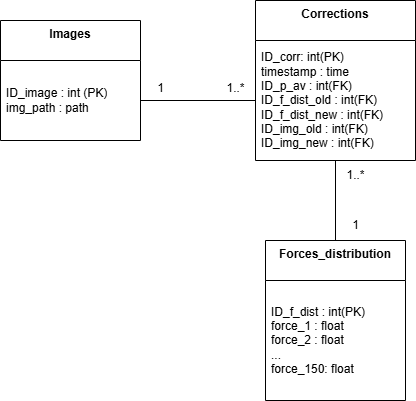
\includegraphics[width=10cm,height=6cm]{figures/db_diagram_corr.png}
\caption{\label{fig:db_corr} Malla Curricular Ingeniería Civil Informática.} Fuente: Elaboración propia.
\end{figure}

Con respecto a los datos adicionales, debido a que estos no cambian con las correcciones, se decide almacenar estos en una tabla propia, conteniendo los atributos clave y sin necesidad de relaciones con otras tablas, como se muestran en la Imágen \ref{fig:db_add_data}.

\begin{figure}[h]
\centering
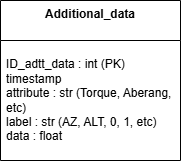
\includegraphics[width=3cm,height=2cm]{figures/db_diagram_add_data.png}
\caption{\label{fig:db_add_data} Malla Curricular Ingeniería Civil Informática.} Fuente: Elaboración propia.
\end{figure}

\subsubsection{Formato de almacenamiento}

Después de diseñar la estructura de los datos, se hace necesario saber qué tecnologías usar para llevarla a cabo.

El modelo relacional de la imágen X entrega la impresión que una base de datos SQL sería la mejor opción. Si bien esta puede permanecer como una opción para futuros usos de los datos extraídos, esta opción no sería óptima para el objetivo de esta memoria, debido a que el procedimiento ETL a desarrollar se acoplara a nivel de código con otros modelos de computación y/o análisis, por lo que subir los datos a un servidor SQL para luego bajarlos en el mismo sistema es redundante e innecesario.

Por ende, y considerando el lenguaje de programación usado (Python 3.10.8), la mejor opción es la librería Pandas, más específicamente la estructura Dataframe, la cuál a nivel técnico es homóloga a una tabla SQL dentro de un ambiente Python.

\subsection{Descripción general del proceso}

El proceso de la solución puede ser revisado en el Anexo 3. Igualmente, el mismo puede resumirse de tres etapas principales, cada una dividida en distintas sub-etapas: 

\begin{enumerate}
    \item Filtrado de líneas de logs:
    En esta etapa, a los registros de log de una noche de operación se les remueven elementos repetidos dentro de las líneas, para luego rescatar las líneas que se encuentren dentro de los periodos de observación ocurridos durante la noche.

    \item Extracción de datos:
    En esta etapa, se extrae la información deseada a las líneas de los registros de log, usando una plantilla de lineas prefabricada, que especifica la ubicación de los datos a extraer dentro de las lineas a leer.

    \item Guardado de datos:
    En esta etapa, se construyen datasets dedicados para uno de los datos a extraer (según discutido en la sección 3.1)  y se ingestan con la información previamente extraída. Luego de esto, se valida que la información ingestada sea consistente y se construyen las relaciones correspondientes entre los datasets.
\end{enumerate}

Los siguientes capítulos se encargan de describir a mayor detalle las etapas del proceso.

\subsection{Filtrado de líneas de log}

Los registros de log poseen cientos de miles de líneas, por lo que un proceso de filtrado aplicado directamente sobre estos sería costoso en tiempo y poder de cómputo.

Por ende, es prudente procesar los registros de log de forma previa, aplicando transformaciones que retornen un conjunto de líneas más apto para el filtrado.

\subsubsection{Remoción de tokens estáticos comunes}

Tras revisar los registros de log, como el ejemplo presente en el Anexo 2, se puede notar que existe un patrón recurrente en todas las líneas.

Estos tokens iniciales, como se menciono en la sección 2.4, aportan información que es redundante dentro de la misma línea y, a su vez, que es estática, ya que la misma no cambia entre las distintas líneas. De este modo, se puede concluir que dicha información no es necesaria para el objetivo de esta memoria.

Por lo mismo, con tal de facilitar la extracción de datos, se procede a eliminar estos tokens estáticos.

\subsubsection{Cruce con archivo de observaciones}

Parte del objetivo de esta memoria es garantizar que la información extraída sea fidedigna y correcta. Por ende, es necesario asegurar que las observaciones a tratar sean exitosas.

Además, no todas las observaciones son usadas en el proceso de Óptica Activa; las observaciones de calibración no son consideradas para este proceso, solo las de adquisición y científicas.

Los registros de log no muestran de qué tipo es cada observación, por ende es necesario extraer esta información de un documento externo y cruzarla con las líneas de observaciones ya extraídas, con tal de así poder obtener las líneas que sí influyen en la Óptica Activa.

\begin{enumerate}

    \item{ESO Observational Raw Data Query}
    
    Como se mencionó en la sección 2.7, la ESO posee una página donde se puede acceder de forma libre a información sobre las observaciones realizadas por el VLT. Dentro de esta información, se puede extraer las observaciones realizadas, la hora en que se realizaron y el tipo de observación, entre otros atributos.
    
    Para obtener el documento de observación necesario para el procedimiento ETL, se deben añadir los campos mostrados en la Imágen \ref{fig:eso_raw}

    \begin{figure}[h]
    \centering
    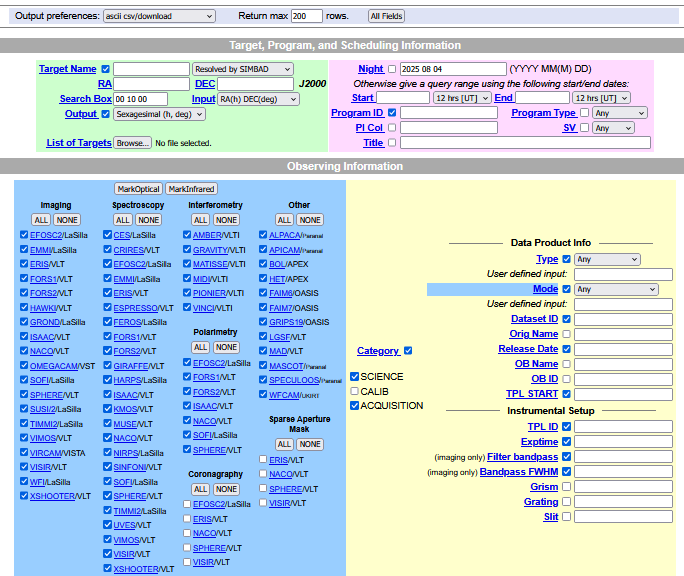
\includegraphics[width=13.5cm,height=9cm]{figures/eso_raw.png}
    \caption{\label{fig:eso_raw} Malla Curricular Ingeniería Civil Informática.} Fuente: Elaboración propia.
    \end{figure}
    
    Estos campos permiten obtener todas las observaciones cientificas y de adquisición de todos los instrumentos en una noche determinada.
    
    Es posible realizar una petición POST con los campos deseados a la página, y esta luego retorna un archivo csv con las observaciones de la noche descrita para todos los instrumentos disponibles durante la misma.

    \item{Segmentación de los periodos de observación}

    Una vez cargado el documento, se procede a usar el mismo para delimitar los horarios de inicio y término de cada periodo de observación valido, para luego usar estos límites en el filtrado de las observaciones obtenidas desde el registro de logs.

    Inicialmente, se pueden crear estos 'bloques de tiempo' usando la hora de inicio de cada observación junto con el tiempo de exposición de la misma. Es importante que, al momento de crear estos bloques, se mantenga la distinción de bajo que instrumento se produce la observación en cuestión.

    Luego de este paso, es natural intuir que algunos de estos bloques para un mismo instrumento se puedan sobrelapar, lo cuál provocaría que se duplicaran algunas líneas de log tras filtrar. Por ende, tras crear los bloques de tiempo, se debe cerciorar que aquellos bloques que se sobrelapen en horario para un mismo instrumento sean unidos.

    Sumado a esto, se conoce que los telescopios estarán en funcionamiento por ciertos intervalos de tiempo previo y posterior a una observación \cite{eso1998vlt}. Por último, se realiza la suposición que entre el fin de un bloque de tiempo y el comienzo del siguiente, la operación del telescopio continua por un lapso de tiempo.
    
    Debido al párrafo anterior, se considera añadir tres margenes paramétricos de tiempo:

    \begin{itemize}
        \item Margen inferior: Cantidad de segundos previo a un bloque de tiempo.

        \item Margen superior: Cantidad de segundos posterior a un bloque de tiempo.

        \item Umbral intermedio: Cantidad de segundos entre bloques de tiempo para un mismo instrumento (con margenes incluidos) donde, si la distancia horaria es menor al umbral, se procede a unir dichos bloques.
        
    \end{itemize}

    Si bien se conoce que cada observatorio es operativo antes y después de una observación formal, la cantidad de tiempo específica (X segundos antes y Z segundos después de cada observación) es desconocida, y no se asegura que sean cantidades estables para cada UT o para una noche específica.

    Es por esta razón, que los margenes y el umbral son paramétricos, con tal de buscar la cantidades bajo las cuales se puede obtener mejores resultados.

    \item{Clasificación según cruce}

    Con los bloques de tiempo formados, solo resta filtrar las líneas de log en base de las mismas.

    Para este proceso, solo basta con incluir todas las líneas de log cuyo horario se encuentre dentro de los bloques de tiempo.

\end{enumerate}

\subsection{Extracción de datos}

El método tradicional para extraer datos de líneas de log es usar plantillas en las mismas. El objetivo es extraer los datos deseados de las líneas de texto, y disponerlos en los formatos adecuados.

Debido a la proliferación y estandarización de este método, se procederá a usar el mismo para las líneas previamente procesadas.

\subsubsection{Plantillas de lineas}

Las plantillas corresponden a una secuencia de carácteres que marcan la posición de los valores deseados dentro de una línea de texto. Debido a que se conoce la cantidad específica de datos requeridos, se decide crear las plantillas manualmente.

Estas plantillas se disponen finalmente al procedimiento ELT, el cuál extraerá los datos de las líneas de log con las plantillas de forma automática.

El formato final de las plantillas varía según el método de extracción de datos usado, por lo que se muestran imágenes de las mismas en las subsecciones correspondientes.

Sin embargo, según el análisis realizado en la sección 3.1, se ha determinado usar 16 plantillas para obtener los datos deseados; una plantilla para cada línea a analizar.

\subsubsection{Extracción de información de las lineas de log}

La extracción de datos de líneas de log se refiere al análisis de las líneas de texto presentes en los registros de log con el fin de identificar los tokens presentes y detectar los datos relevantes con el fin de extraerlos \cite{jayathilake2011mind}. 

Existen varias formas de realizar la extracción de datos en registros de log; escoger la adecuada no es trivial, ya que se presentan dos desafíos principales a la hora de aplicar la misma en logs \cite{jayathilake2011mind}:

Las arquitecturas de software grandes y complejas generan grandes cantidades de información de log mientras se ejecutan, por lo que la forma tradicional de construir manualmente expresiones regulares es demasiado costosa.
Las funciones de sistemas de software complejos y actualizaciones de negocio de alta frecuencia llevan a actualizaciones más frecuentes de plantillas de línea, incrementado así en gran medida la diversidad de plantillas de línea.

La problemática 1 se orienta principalmente a la extracción de datos general de registros de log, el cuál no es el caso para este trabajo; ya que se tiene claridad de los datos requeridos y de las líneas específicas que los poseen, el uso de expresiones regulares y plantillas creadas manualmente no es descartado.

La problemática 2, si bien también se orienta hacia la extracción de datos general de registros de log y a la creación automática de plantillas de log, se puede extender su cuestionamiento a la creación de plantillas manuales; a medida que se actualicen las reglas de negocio de la Óptica Activa, las plantillas manuales creadas pueden aumentar.

Como se mencionó en el Capítulo 1, el sistema de logging de Óptica Activa tiene décadas de servicio continuo, por lo que es poco probable que se realicen cambios en esta área. Por el lado de los datos relevantes para el sistema de Óptica Activa, es posible que puedan existir cambios en los datos requeridos en un futuro, sin embargo el análisis realizado en la sección 3.1, se puede asegurar que los cambios se mantendrían dentro de ese modelo de datos. Por ende, cualquier cambio futuro no incrementa el número de plantillas en gran medida.

Debido a todo lo anterior, se decide optar por un modelo sencillo de extracción de datos en líneas de log, donde se itera sobre las secciones de log obtenidas tras el preprocesamiento, y dentro de cada iteración se aplica de forma greedy cada plantilla sobre la línea seleccionada hasta que una calce. En caso de calzar, se extraen los datos acordes a la plantilla y se almacenan estos en una lista.

Para aplicar la extracción de datos en las líneas de texto, existen varios métodos y librerías diseñadas para la extracción de datos desde strings. Para este trabajo, se analizaron dos opciones posibles y se compararon según eficiencia y exactitud.

\begin{enumerate}

    \item{Extracción de datos con Expresiones Regulares}
    
    En este caso, se tienen las plantillas en forma de expresiones regulares, donde los tokens deseados estan marcados como grupos dentro de las mismas plantillas.

    Para este caso, se iteran en todas las líneas de log filtradas por observación, y se detectan las líneas que contienen los datos deseados usando ciertos tokens claves detectados al estudiar el formato del archivo de log.

    Luego de detectar las líneas, se aplican a estas todas las plantillas hasta que se pueda extraer correctamente con una.

    Para este método de extracción, las plantillas tienen el formato presentado en el Listing \ref{myverbatim:regex}:

    \begin{myverbatim}[caption={Plantillas Regex},label={myverbatim:regex}]

(([0-2][0-9]{3}-[0-1][0-9]-[0-3][0-9]) ([0-2][0-9]:
[0-5][0-9]:[0-5][0-9](.[0-9]+)*) lt[1-4]m1m3 m1as 
m1asSetGlb[Abs|Rel]+ [0-9.-]+ [0-9.-]+ AS Forces 
#([0-9.-]+) \(abs\): ([0-9.\-\s]+))

(([0-2][0-9]{3}-[0-1][0-9]-[0-3][0-9]) ([0-2][0-9]:
[0-5][0-9]:[0-5][0-9](.[0-9]+)*) lt[1-4]m1m3 m1as 
m1asSetGlb[Abs|Rel]+ [0-9.-]+ [0-9.-]+ AS Executed 
cmd #([0-9.-]+): SUCCESS)

(([0-2][0-9]{3}-[0-1][0-9]-[0-3][0-9]) ([0-2][0-9]:
[0-5][0-9]:[0-5][0-9](.[0-9]+)*) lt[1-4]m1m3 m1as 
m1asSetGlb[Abs|Rel]+ [0-9.-]+ [0-9.-]+ AS Received 
cmd #([0-9.-]+): [A-Z]+)

(wt[1-4]tcs ([0-2][0-9]:[0-5][0-9]:[0-5][0-9]
(.[0-9]+)*)> DET EXP NO = ([0-9]+) \/ Unique exposure 
ID number \[(lt[1-4][a-z]{2}[a-c])\])

(wt[1-4]tcs ([0-2][0-9]:[0-5][0-9]:[0-5][0-9]
(.[0-9]+)*)> TEL ACTO (INTTIME) = ([0-9]+))

(wt[1-4]tcs ([0-2][0-9]:[0-5][0-9]:[0-5][0-9]
(.[0-9]+)*)> TEL (ALT) (TORQUE) = ([0-9.-]+))

(wt[1-4]tcs ([0-2][0-9]:[0-5][0-9]:[0-5][0-9]
(.[0-9]+)*)> TEL (AZ) (TORQUE) = ([0-9.-]+))

(wt[1-4]tcs ([0-2][0-9]:[0-5][0-9]:[0-5][0-9]
(.[0-9]+)*)> TEL (ALT)( )= ([0-9.-]+))

(wt[1-4]tcs ([0-2][0-9]:[0-5][0-9]:[0-5][0-9]
(.[0-9]+)*)> TEL (AZ)( )= ([0-9.-]+))

(wt[1-4]tcs ([0-2][0-9]:[0-5][0-9]:[0-5][0-9]
(.[0-9]+)*)> TEL (IA) (ABER)([0-9.-]+) = ([0-9.-]+))

(wt[1-4]tcs ([0-2][0-9]:[0-5][0-9]:[0-5][0-9]
(.[0-9]+)*)> TEL (IA) (ABERANG)([0-9.-]+) = ([0-9.-]+))

(wt[1-4]tcs ([0-2][0-9]:[0-5][0-9]:[0-5][0-9]
(.[0-9]+)*)> TEL (ACTO) (ALTPOS) = ([0-9.-]+))

(wt[1-4]tcs ([0-2][0-9]:[0-5][0-9]:[0-5][0-9]
(.[0-9]+)*)> TEL (ACTO) (AZPOS) = ([0-9.-]+))

(wt[1-4]tcs ([0-2][0-9]:[0-5][0-9]:[0-5][0-9]
(.[0-9]+)*)> TEL (IA) (ABERAVE)([0-9.-]+) = ([0-9.-]+))

(wt[1-4]tcs ([0-2][0-9]:[0-5][0-9]:[0-5][0-9]
(.[0-9]+)*)> TEL (IA) (ABERAVEANG)([0-9.-]+) = 
([0-9.-]+))

(wt[1-4]tcs ([0-2][0-9]:[0-5][0-9]:[0-5][0-9]
(.[0-9]+)*)> TEL (IA) (ABERFILMOD)([0-9.-]+) = 
([0-9.-]+))

(wt[1-4]tcs ([0-2][0-9]:[0-5][0-9]:[0-5][0-9]
(.[0-9]+)*)> TEL (IA) (ABERFILANG)([0-9.-]+) = 
([0-9.-]+))
    
    \end{myverbatim}

    \item{Extracción de datos con Template Text Parser}

    Para este caso, se usa la librería externa Template Text Parser, o TTP, la cuál, de forma similar al caso anterior, permite escribir los tokens deseados en la misma plantilla, y luego durante la extracción solo retorna los datos llamados anteriormente.

    Como es una librería diseñada para estos fines exclusivos, se procede solo a ejecutar un método de la misma para extraer datos.

    Para este método de extracción, las plantillas tienen el formato presentadas en el Listing \ref{myverbatim:ttp}:

    \begin{myverbatim}[caption={Plantillas TTP},label={myverbatim:ttp}]

{{ date }} {{ hour }} lt[1-4]m1m3 m1as m1asSetGlbAbs 
[0-9.-]+ [0-9.-]+ AS Forces #([0-9.-]+) \(abs\): 
{{ data }}

{{ date }} {{ hour }} lt[1-4]m1m3 m1as m1asSetGlbAbs 
[0-9.-]+ [0-9.-]+ AS Executed cmd #([0-9.-]+): SUCCESS

{{ date }} {{ hour }} lt[1-4]m1m3 m1as m1asSetGlbAbs 
[0-9.-]+ [0-9.-]+ AS Received cmd #([0-9.-]+): [A-Z]+

wt[1-4]tcs {{ hour }}> DET EXP NO = ([0-9]+) \/ Unique 
exposure ID number \[(lt[1-4][a-z]{2}[a-c])\]

wt[1-4]tcs {{ hour }}> TEL ACTO (INTTIME) = ([0-9]+)

wt[1-4]tcs {{ hour }}> TEL {{ group }} >{{ label }} = 
{{ data }}

wt[1-4]tcs {{ hour }}> TEL {{ group }} {{ label }} = 
{{ data }}

wt[1-4]tcs {{ hour }}> TEL {{ group }}{{ label }}= 
{{ data }}

wt[1-4]tcs {{ hour }}> TEL {{ group }}{{ label }}= 
{{ data }}

wt[1-4]tcs {{ hour }}> TEL {{ group }} {{ label }} = 
{{ data }}
    
    \end{myverbatim}

\end{enumerate}

Para ambos casos, los datos extraídos quedan en formato json, donde la llave corresponde al nombre de la caracteristica (definida desde la plantilla con TTP y definida desde el codigo con Regex) y el valor corresponde al dato extraído.

Independiente del origen del dato, todos poseen campos de nombre 'group' y la mayoría posee también un campo 'label'. Se usará el campo 'group' para definir el tipo del dato (distribución de fuerza, imágen, etc.) y el campo 'label' para identificar subdivisiones dentro de cada tipo de dato cuando sea conveniente.

Estos campos se tornan particularmente útiles, cuando se considera que la información para un dato puede estar repartida en varias líneas, como es por ejemplo el caso de las distribuciones de fuerza, donde las fuerzas de los 150 actuadores están siempre repartidos en 6 líneas de 25 actuadores, y que a su vez todas esas líneas están separadas de la ID de la distribucón, que se encuentra en su línea propia. Este formato se puede revisar en el ejemplo disponible en el Anexo 4.

De esta forma, mediante el uso de estos campos, se puede dejar registro de la información de un mismo dato para su posterior unión.

\subsection{Guardado de los datos}

Una vez extraídos los datos, se deben crear y validar los dataframes donde se almacenaran estos mismos, siguiendo la filosofía descrita en la sección 3.2.

Es necesario no solo crear los dataframes de forma coherente, sino que también validar que los datos ingresados sean correctos ya sea en formato, en contexto, etc.

\subsubsection{Construcción de los dataframes}

En la sección 3.2.1. se definieron las tablas a desarrollar con sus relaciones y atributos correspondientes, por ende, los dataframes a crear deben seguir la misma estructura.

Asi mismo, se crearan 4 dataframes:

\begin{itemize}

    \item Uno para las instancias de corrección, donde para cada instancia se guardan las referencias a las imágenes y distribuciones de fuerza anteriores y posteriores.

    \item Uno para las distribuciones de fuerza, donde para cada distribución se guardan los pesos de los 150 actuadores y el timestamp del registro en el log.

    \item Uno para las imágenes tomadas, donde para cada imágen se guardan los tiempos de inicio y término de lectura, el tiempo de inicio de exposición, el tiempo de integración, el sensor que leyo la imágen y la dirección local al archivo .fits correspondiente.

    \item Uno para todos los datos adicionales, donde para cada dato se guarda el grupo (relacionado con la cantidad con la que trata, ya sea altitud, acimut, imágen, etc.), la etiqueta (relacionado con la cualidad específica que maneja esa cantidad, sean aberraciones, torque, etc.), el dato numérico o en texto. Para lo último, se decide guardar el dato en formato entero, flotante y texto, con fines de respaldo, sumado a un campo de tipo de dato que describe cuál es el formato correcto.
    
\end{itemize}

De esta forma, los dataframes finales poseen los mismos esquemas que los presentados en el diagrama de la sección 3.2.1.

\subsubsection{Ingesta a los dataframes}

Debido a que los datos extraídos se encuentran en formato json, corresponde iterar por todos los datos, y migrar los datos desde el formato json a dataframe.

En la sección 3.4.2. se mencionaron las llaves 'group' y 'label' para diferenciar los tipos de datos. Estas llaves se usan en este proceso, con tal de poder identificar el tipo de dato, y según aquello, migrar los datos de forma acorde.

Como ejemplo, se conoce que los datos de distribución de fuerzas posee un campo con las fuerzas de los actuadores, y que ningún otro tipo de dato posee tal campo. Entonces, al tener registro del tipo de dato en la llave 'group', se puede validar que datos poseen ese campo y extraerlos sin temor a falla.

Asi mismo, se puede concatenar la información de ciertos datos que se encontraban en múltiples líneas. Tras revisar el campo 'group', se revisa que no existan datos en el dataframe con información faltante, y se revisa el campo 'label' para verificar que tipo de información específica es la que falta.

\subsubsection{Validación de los dataframes}

Eventualmente durante el proceso de ingesta a los dataframes se producirán errores, principalmente por errores en los datos desde el origen o por las convenciones tomadas para el desarrollo de los filtros.

Debido a ello, luego de la ingesta, se deben validar los datos dentro de los dataframes con tal de asegurar que dicha información es correcta y de útilidad.

Para cada tipo de dato, el proceso de validación es distinto:

\begin{itemize}
    \item Para las instancias de corrección, se deben remover las instancias con ID nulo, y también se remueven aquellas instancias que no poseen distribución de fuerza posterior a la corrección.

    \item Para las distribuciones de fuerza, se deben remover las instancias con ID nulo y también se remueven aquellas distribuciones que no son antecedidas y/o seguidas por imágenes únicas.

    \item Para las imágenes, solo se remueven las instancias con ID nulo.
\end{itemize}

El dataframe de additional-data no es validado, debido a ser datos de carácter miscelaneo y secundario.

\subsubsection{Relación de los dataframes}

Finalmente, una vez se valida la información presente en los dataframes, se procede a crear las relaciones mencionadas en la sección 3.2.2.

Para esto, simplemente se hacen calzar los timestamp de los datos de imágen y de distribución de fuerza, y luego se entrega sus ID a la instancia de corrección para incluirlas en sus campos de llaves foráneas.